\documentclass[11pt]{article}

% ---------------------------------------------------------------------------
%  OncoEvidence -- final project deliverable (completed-project report)
%  Compile with:  tectonic docs/deliverable.tex
%  Every number is taken from results/*.json in this repository.
% ---------------------------------------------------------------------------

\usepackage[margin=1in]{geometry}
\usepackage{amsmath,amssymb}
\usepackage{xcolor}
\usepackage{tikz}
\usetikzlibrary{arrows.meta,positioning,fit,backgrounds,calc,shapes.geometric}
\usepackage{booktabs}
\usepackage{array}
\usepackage{colortbl}
\usepackage[most]{tcolorbox}
\usepackage{enumitem}
\usepackage{graphicx}
\usepackage{float}
\usepackage{caption}
\captionsetup{font=small,labelfont=bf}
\graphicspath{{../figures/}{figures/}}

% ----- Palette -------------------------------------------------------------
\definecolor{sriblue}{HTML}{1F4E79}
\definecolor{sriaccent}{HTML}{E8684A}
\definecolor{srigreen}{HTML}{2E8B57}
\definecolor{srigray}{HTML}{4B5563}
\definecolor{srilight}{HTML}{EAF1F8}
\definecolor{sriamber}{HTML}{F6BD16}
\definecolor{srirow}{HTML}{F2F6FB}
\definecolor{srired}{HTML}{C0392B}
\definecolor{nDrug}{HTML}{E8684A}
\definecolor{nGene}{HTML}{2E8B57}
\definecolor{nPath}{HTML}{F6BD16}
\definecolor{nDis}{HTML}{5B8FF9}

\usepackage[colorlinks=true,linkcolor=sriblue,citecolor=sriblue,urlcolor=sriaccent]{hyperref}

\usepackage{titlesec}
\titleformat{\section}{\large\bfseries\color{sriblue}}{\thesection}{0.6em}{}
\titleformat{\subsection}{\normalsize\bfseries\color{sriblue!85!black}}{\thesubsection}{0.5em}{}
\titlespacing*{\section}{0pt}{1.5ex}{0.8ex}

\newtcolorbox{problembox}{colback=srilight,colframe=sriblue,boxrule=0.9pt,
  arc=2pt,left=6pt,right=6pt,top=5pt,bottom=5pt}
\newtcolorbox{winbox}{colback=sriaccent!8,colframe=sriaccent,boxrule=0.9pt,
  arc=2pt,left=6pt,right=6pt,top=5pt,bottom=5pt}
\newtcolorbox{nullbox}{colback=srigray!8,colframe=srigray,boxrule=0.9pt,
  arc=2pt,left=6pt,right=6pt,top=5pt,bottom=5pt}
\newtcolorbox{findbox}[1]{colback=srigreen!7,colframe=srigreen,boxrule=0.8pt,
  arc=2pt,left=6pt,right=6pt,top=4pt,bottom=4pt,title={#1},
  fonttitle=\bfseries\color{white},colbacktitle=srigreen}

\renewcommand{\arraystretch}{1.22}
\newcommand{\NN}{\mathcal{N}}
\newcommand{\zd}{\mathbf{z}}

\begin{document}

\begin{center}
  {\LARGE\bfseries\color{sriblue} OncoEvidence: Mechanism-Guided Evidence\\ Triage for Cancer Drug Repurposing}\\[4pt]
  {\large\bfseries\color{sriblue!80!black} When a knowledge graph earns its place, and how to show its\\ mechanism reasoning is predictive and faithful}\\[10pt]
  {\large Akshatha Arunkumar}\\[2pt]
  {\small Final Project Deliverable \quad\textbar\quad \today}
\end{center}

\vspace{2pt}
\begin{problembox}
\textbf{Abstract.} OncoEvidence ranks oncology drug-repurposing candidates on the
PrimeKG knowledge graph, extracts the multi-hop mechanism path that would explain each
one, and uses a literature-grounded language model to grade whether that mechanism is
supported. The project is built around an honest question: once a strong tabular ranker
is in place, what does the graph actually add? We show the answer is \emph{mechanism},
and we then stress that mechanism signal along the two axes that matter for a real
triage tool. On a corrected, leakage-safe benchmark (5 seeds) a tuned XGBoost matches or
beats the graph network at link ranking. But only the graph yields a traceable
drug\,$\to$\,target\,$\to$\,cancer-gene\,$\to$\,cancer path; that path structure
separates true indications from random pairs at AUROC 0.879 and agrees with curated
DrugMechDB at 0.802. Two new results make the case stronger. On a prospective time-split
the graph model ranks \emph{future} oncology indications at AUROC 0.930 and beats a
structure-blind control by $+0.047$; concretely, trained only on pre-2005 structure it
surfaces $11\times$ as many future indications in the top 50 as the control, including
post-cutoff approvals like romidepsin and pralatrexate for cutaneous T-cell lymphoma and
nilotinib for CML. And a counterfactual test shows the mechanism head is \emph{faithful}:
deleting the curated mechanism edge, and only that edge, collapses the prediction
($p\approx3.6\times10^{-34}$). An orthogonal check against ClinicalTrials.gov is reported as
a fully characterized negative: after removing both drug and cancer popularity, the
interaction signal vanishes (AUROC 0.475).
\end{problembox}

\begin{winbox}
\textbf{Six findings at a glance.}
\begin{enumerate}[leftmargin=1.4em,itemsep=0pt,topsep=2pt]
\item Plain link ranking does not need the graph: tuned XGBoost matches or beats the GNN in every regime.
\item Only the graph produces a traceable multi-hop mechanism path.
\item Mechanism structure separates true indications from random pairs (AUROC 0.879) and matches DrugMechDB (0.802); honest under hard negatives --- strong vs random/oncology-drug (0.887/0.870), modest (0.609) under the hardest shared-target controls.
\item Blinded mechanism recovery: with the direct edge hidden, the \emph{jointly-supervised} GNN names the bridge gene (R@10 0.25) where degree-trivial and link-only baselines hit $\sim$0 --- the mechanism objective, not architecture alone, creates the signal.
\item \textbf{New, prospective:} on a time-split the GNN ranks future indications at AUROC 0.930 (vs sampled negatives) and \emph{enriches the top-priority tail} --- $11\times$ as many future indications in the top 50 as a structure-blind control (named post-2005 approvals included), though it is not better on median rank.
\item \textbf{New, faithfulness:} deleting the curated mechanism edge hurts $\gg$ a random edge (contrast 0.124, $p\approx3.6\times10^{-34}$, faithful 83\%).
\end{enumerate}
\end{winbox}

% ===========================================================================
\section{Background and significance}

Developing a new drug takes many years and large cost, while thousands of approved drugs
already carry known safety profiles. If an approved drug acts on a protein or pathway
that also drives a cancer, repurposing it is a fast route to a candidate therapy.
Biomedical knowledge graphs such as PrimeKG encode millions of relationships among drugs,
proteins, genes, pathways, and diseases, so the information needed to reason about such
mechanisms already exists as paths through the graph. The open problem is \emph{trust}: a
bare drug-disease score hides its reasoning and cannot separate a real mechanism from a
coincidence.

\textbf{Novelty, stated carefully.} Knowledge-graph repurposing with explanations is not
new: TxGNN~\cite{txgnn} is a graph foundation model with multi-hop rationales, and
KGML-xDTD~\cite{kgmlxdtd} predicts treatment links with KG-based mechanism paths. This
project does not claim ``a knowledge graph plus a language model for repurposing'' as
novel. The defensible contribution is methodological: quantify \emph{when} graph
structure adds value beyond a strong tabular ranker, show that its value is mechanism
extraction rather than better ranking, and audit those mechanisms three ways most demos
skip --- against a curated mechanism database, against a prospective time-split, and
against a counterfactual faithfulness test.

% ===========================================================================
\section{Data and system}

\textbf{Knowledge graph.} We use PrimeKG~\cite{primekg}, processed into a heterogeneous
graph of 129{,}312 nodes and 8{,}100{,}498 directed edges over 50 relation types
(Table~\ref{tab:nodes}). The prediction target is the
drug\,$\xrightarrow{\text{indication}}$\,disease relation (9{,}388 edges), with 3{,}170
oncology diseases flagged by an ontology-keyword filter.

\begin{table}[H]
\centering\small
\begin{tabular}{>{\raggedright\arraybackslash}p{0.27\linewidth} r r | >{\raggedright\arraybackslash}p{0.27\linewidth} r r}
\toprule
\rowcolor{sriblue}\color{white}\textbf{Node type} & \color{white}\textbf{Count} & \color{white}\textbf{dim} & \color{white}\textbf{Node type} & \color{white}\textbf{Count} & \color{white}\textbf{dim}\\
\midrule
\rowcolor{srirow} biological\_process & 28{,}642 & 384 & disease & 17{,}080 & 384\\
gene / protein & 27{,}610 & 384 & effect\_phenotype & 15{,}311 & 384\\
\rowcolor{srirow} anatomy & 14{,}033 & 384 & molecular\_function & 11{,}169 & 384\\
drug & 7{,}957 & 384 & pathway & 2{,}516 & 384\\
\rowcolor{srirow} cellular\_component & 4{,}176 & 384 & exposure & 818 & 384\\
\bottomrule
\end{tabular}
\caption{PrimeKG node inventory. Every node carries a 384-d SentenceTransformer
embedding of its name, shared identically by the GNN and the tabular baselines so that
any performance gap measures graph structure, not features.}
\label{tab:nodes}
\end{table}

\begin{figure}[H]
\centering
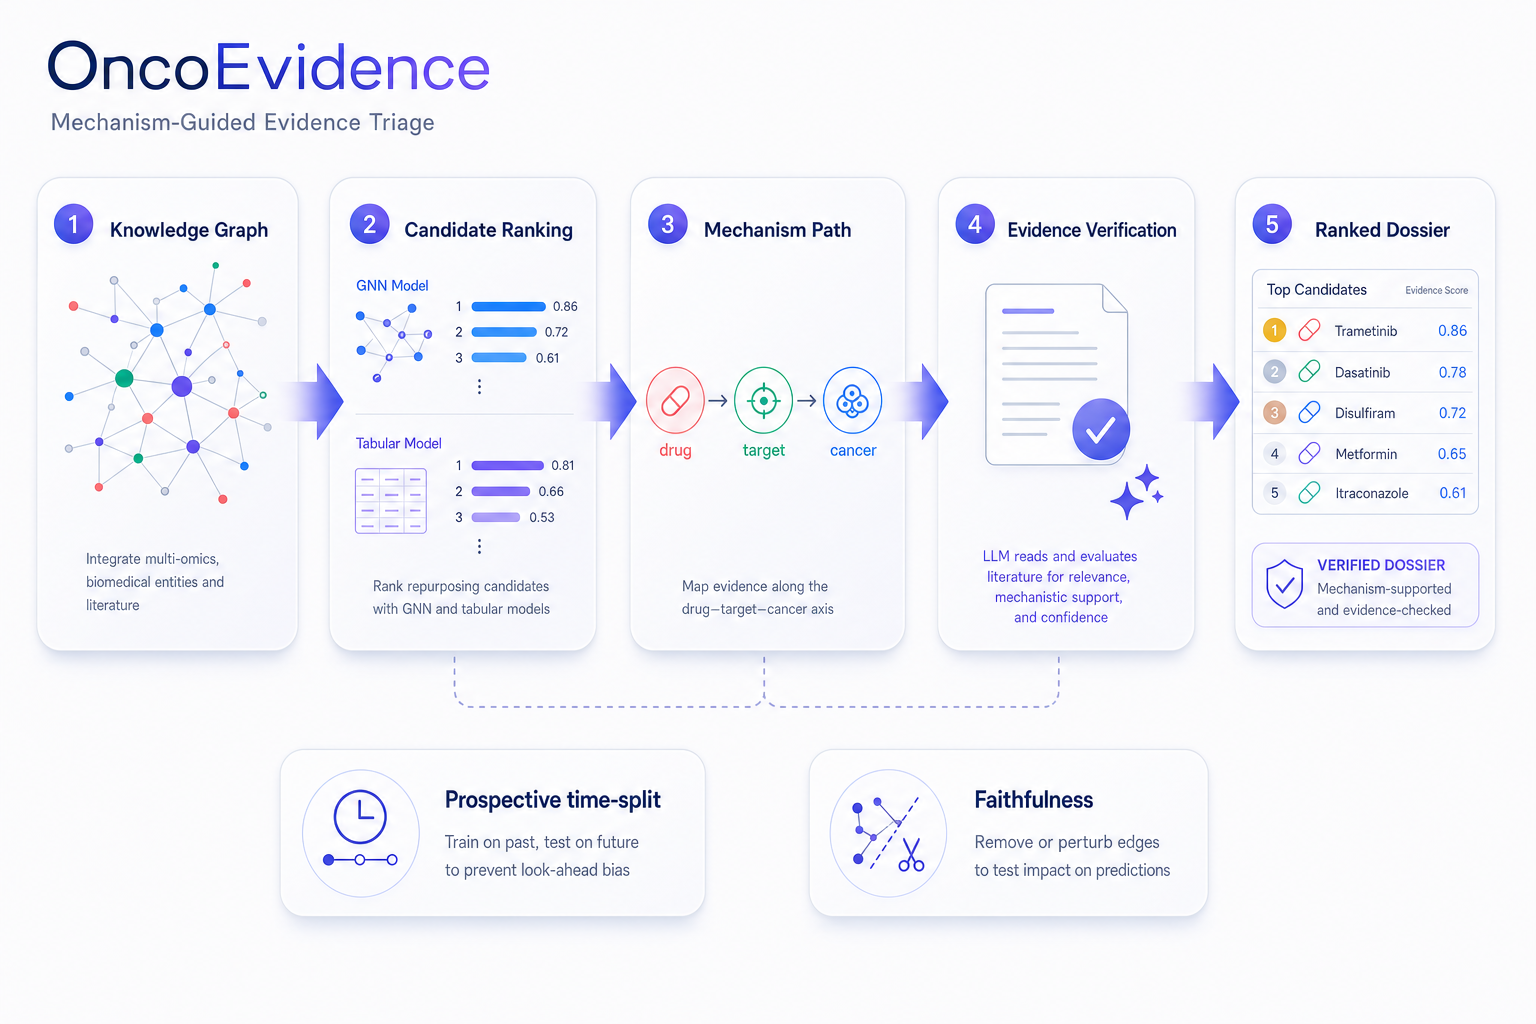
\includegraphics[width=\linewidth]{oncoevidence_main_diagram.png}
\caption{The OncoEvidence pipeline. We rank drug--disease candidates over PrimeKG,
extract a multi-hop mechanism path (drug $\to$ target $\to$ cancer gene $\to$ cancer),
verify it against Europe PMC abstracts with an LLM, and emit an evidence-backed ranked
dossier. Two audits stress-test the system: a prospective time-split (train on past,
test on future) and a counterfactual faithfulness test (remove mechanistic edges and
re-evaluate).}
\label{fig:pipeline}
\end{figure}

% ===========================================================================
\section{Methods}

\subsection{Candidate ranking and the controls}
Repurposing is framed as link prediction on the drug\,$\to$\,indication\,$\to$\,disease
relation. A heterogeneous GraphSAGE~\cite{sage} encoder builds an embedding for every
node by message passing over its typed neighbours, and an MLP decoder scores a pair:
\begin{equation}
\mathbf{h}_v^{(l)} = \sigma\!\Big( W^{(l)}\big[\,\mathbf{h}_v^{(l-1)}\ \big\Vert\
\textstyle\operatorname*{AGG}_{u\in\NN_r(v)} \mathbf{h}_u^{(l-1)}\big]\Big),
\qquad
s(d,c) = \mathrm{MLP}\big(\big[\,\zd_d \,\Vert\, \zd_c\,\big]\big).
\label{eq:gnn}
\end{equation}
Three controls receive the \emph{same} features: a tuned XGBoost on the concatenated
endpoint features (the primary tabular ranker), a \textsc{FeatureMLP} (the same projection
and decoder but no message passing), and a DistMult knowledge-graph embedding
$s(d,c)=\zd_d^\top \mathrm{diag}(\mathbf{r})\,\zd_c$ (a pure memorizer with no
representation for unseen nodes). All models are trained with binary cross-entropy on
positives and sampled negatives.

\subsection{Mechanism-path extraction}
For a candidate we search PrimeKG for short paths through mechanism relations
(drug-target, protein-protein, protein-pathway, protein-disease), scoring each by
specificity and penalizing promiscuous hubs:
\begin{equation}
\mathrm{score}(p) \;=\; \beta_{\text{type}} \;+\;
\underbrace{\frac{1}{\log_2(\deg(\text{bridge})+2)}}_{\text{bridge specificity}}\cdot
\underbrace{\frac{1}{\log_2(\delta_{\text{drug}}+2)}}_{\text{IDF carrier penalty}},
\label{eq:mech}
\end{equation}
where $\delta_{\text{drug}}$ is the number of drugs that bind the bridge protein (an
inverse-frequency penalty that suppresses generic carriers such as albumin) and
$\beta_{\text{type}}$ orders direct-target ($3$) over interaction ($2$) over
shared-pathway ($1$) templates. A typical recovered chain:

\begin{figure}[H]
\centering
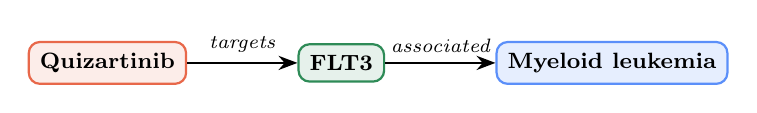
\begin{tikzpicture}[
  >={Stealth[length=2.4mm]}, node distance=6mm and 14mm,
  drug/.style={rounded corners,draw=nDrug,fill=nDrug!12,thick,font=\footnotesize\bfseries,inner sep=4pt},
  gene/.style={rounded corners,draw=nGene,fill=nGene!12,thick,font=\footnotesize\bfseries,inner sep=4pt},
  dis/.style={rounded corners,draw=nDis,fill=nDis!15,thick,font=\footnotesize\bfseries,inner sep=4pt}]
  \node[drug] (d) {Quizartinib};
  \node[gene,right=of d] (g) {FLT3};
  \node[dis,right=of g] (c) {Myeloid leukemia};
  \draw[->,thick] (d) -- node[above,font=\scriptsize\itshape]{targets} (g);
  \draw[->,thick] (g) -- node[above,font=\scriptsize\itshape]{associated} (c);
\end{tikzpicture}
\caption{A direct-target mechanism path. The extractor recovers textbook MOAs such as
Quizartinib--FLT3, Tamibarotene--RARA, Topotecan--TOP1, and Trifluridine--TYMS for true
indications; random pairs usually yield no path.}
\label{fig:mechpath}
\end{figure}

\subsection{The deliverable: a mechanism-grounded candidate dossier}
The deployment artifact (\texttt{scripts/generate\_report.py}) is deliberately
\emph{mechanism-first}, not score-first. For each cancer we rank novel drugs by
disease-specific lift and then \emph{keep only} candidates for which the graph yields a real
MOA path; phenotype/symptom coincidences are dropped by construction, so the list never
contains rationales like ``drug $\to$ fatigue $\leftarrow$ cancer''. Table~\ref{tab:dossier}
shows representative rows. When a cancer has no mechanism-backed novel candidate in the pool,
we say so rather than pad the list --- the graph has to earn each entry. This is
hypothesis-generating triage, not a vetted clinical recommendation.

\begin{table}[H]
\centering\small
\begin{tabular}{>{\raggedright\arraybackslash}p{0.20\linewidth} >{\raggedright\arraybackslash}p{0.20\linewidth} >{\raggedright\arraybackslash}p{0.34\linewidth} c}
\toprule
\rowcolor{sriblue}\color{white}\textbf{Cancer} & \color{white}\textbf{Candidate} & \color{white}\textbf{Top MOA path (direct target)} & \color{white}\textbf{Lift}\\
\midrule
\rowcolor{srirow} glioblastoma & Tamoxifen & Tamoxifen $\to$ PRKCA $\leftarrow$ glioblastoma & $+0.67$\\
glioblastoma & Liothyronine & Liothyronine $\to$ PCNA $\leftarrow$ glioblastoma & $+0.67$\\
\rowcolor{srirow} metastatic melanoma & Pimecrolimus & Pimecrolimus $\to$ MTOR $\leftarrow$ melanoma & $+0.76$\\
prostate cancer & Pamidronic acid & Pamidronic acid $\to$ CASP9 $\leftarrow$ prostate cancer & $+0.83$\\
\rowcolor{srirow} prostate cancer & Zinc chloride & Zinc chloride $\to$ MDM2 $\leftarrow$ prostate cancer & $+0.83$\\
\bottomrule
\end{tabular}
\caption{Mechanism-grounded candidate dossier (excerpt from
\texttt{results/repurposing\_shortlist.md}). Every row carries a target/PPI/pathway MOA path;
non-mechanistic phenotype bridges are excluded. Candidates are novel (no existing indication
edge) and ranked by disease-specific lift. Hypothesis-generating only.}
\label{tab:dossier}
\end{table}

\subsection{The mechanism head and the joint objective}
A mechanism head scores a (drug, gene, disease) triple on the \emph{same} encoder
embeddings, $s_{\text{mech}}(d,g,c)=\mathrm{MLP}\big([\zd_d\Vert\zd_g\Vert\zd_c]\big)$.
We train it jointly with the link objective using an InfoNCE term that ranks the curated
DrugMechDB bridge gene $g^{+}$ above $K$ degree-matched decoys $g^{-}_k$:
\begin{equation}
\mathcal{L} = \mathcal{L}_{\text{link}} + \lambda\,\mathcal{L}_{\text{mech}},
\qquad
\mathcal{L}_{\text{mech}} = -\log
\frac{\exp s_{\text{mech}}(d,g^{+},c)}
     {\exp s_{\text{mech}}(d,g^{+},c)+\sum_{k=1}^{K}\exp s_{\text{mech}}(d,g^{-}_k,c)}.
\label{eq:infonce}
\end{equation}

\subsection{The two audits: prospective and faithfulness}
\textbf{Prospective (temporal) split.} PrimeKG has no timestamps, so we assign each true
oncology pair $(d,c)$ an approximate first-evidence year $\tau(d,c)$ = earliest Europe PMC
co-mention. For a cutoff $T$, the PAST set $\{(d,c):\tau\le T\}$ seeds the
message-passing graph and supervision, while the FUTURE set $\{(d,c):\tau> T\}$ is held
out; its target edges are removed, so the model must rank future indications above
negatives using only pre-$T$ structure.

\textbf{Counterfactual faithfulness.} For a held-out pair whose bridge gene $g$ is a real
drug-target edge $e_{dg}$, we recompute $g$'s mechanism score after deleting $e_{dg}$ and
compare against deleting a random other target edge $e_{dr}$ of the same drug:
\begin{equation}
\Delta_{\text{MOA}} = s_{\text{full}} - s_{\setminus e_{dg}},\quad
\Delta_{\text{rand}} = s_{\text{full}} - s_{\setminus e_{dr}},\quad
\text{contrast} = \overline{\Delta_{\text{MOA}}} - \overline{\Delta_{\text{rand}}}.
\label{eq:faith}
\end{equation}
A faithful model satisfies $\Delta_{\text{MOA}}\gg\Delta_{\text{rand}}$.

\subsection{Metrics}
We report AUROC and AUPRC for separation/ranking, recall@$k$ for retrieval, and the
precision of ``supported'' verdicts,
\begin{equation}
\text{precision} =
\frac{\#\{\text{``supported'' pairs whose path gene is in the DrugMechDB MOA set}\}}
     {\#\{\text{``supported'' pairs DrugMechDB covers}\}}.
\label{eq:prec}
\end{equation}

% ===========================================================================
\section{Results}

\subsection{Finding 1: the link task does not need the graph}
With a tuned XGBoost on shared features, the GNN does not win in any regime
(Table~\ref{tab:bench}, Fig.~\ref{fig:bench}). Paired tests confirm it: in the
cold-disease regime XGBoost beats the GNN by 0.081 AUROC (the GNN-favoring one-sided test
gives $p=0.98$), while the GNN crushes the DistMult memorizer ($+0.43$ AUROC,
$p=2.4\times10^{-4}$). For link ranking with rich text features, a strong tabular model
suffices.

\begin{table}[H]
\centering\small
\begin{tabular}{>{\raggedright\arraybackslash}p{0.30\linewidth} cccc}
\toprule
\rowcolor{sriblue}\color{white}\textbf{Test AUROC (5 seeds)} & \color{white}\textbf{GNN} & \color{white}\textbf{XGBoost} & \color{white}\textbf{MLP} & \color{white}\textbf{KGE}\\
\midrule
\rowcolor{srirow} Transductive & 0.977 & \textbf{0.988} & 0.973 & 0.907\\
Inductive (cold-disease, oncology) & 0.882 & \textbf{0.963} & 0.930 & 0.452\\
\rowcolor{srirow} Inductive (cold-drug) & 0.956 & \textbf{0.958} & 0.931 & 0.482\\
\bottomrule
\end{tabular}
\caption{Corrected, leakage-safe benchmark (mean over 5 seeds). The DistMult memorizer
(KGE) collapses on unseen nodes in both inductive regimes, confirming the task needs
content features, not memorized identity.}
\label{tab:bench}
\end{table}

\begin{figure}[H]
\centering
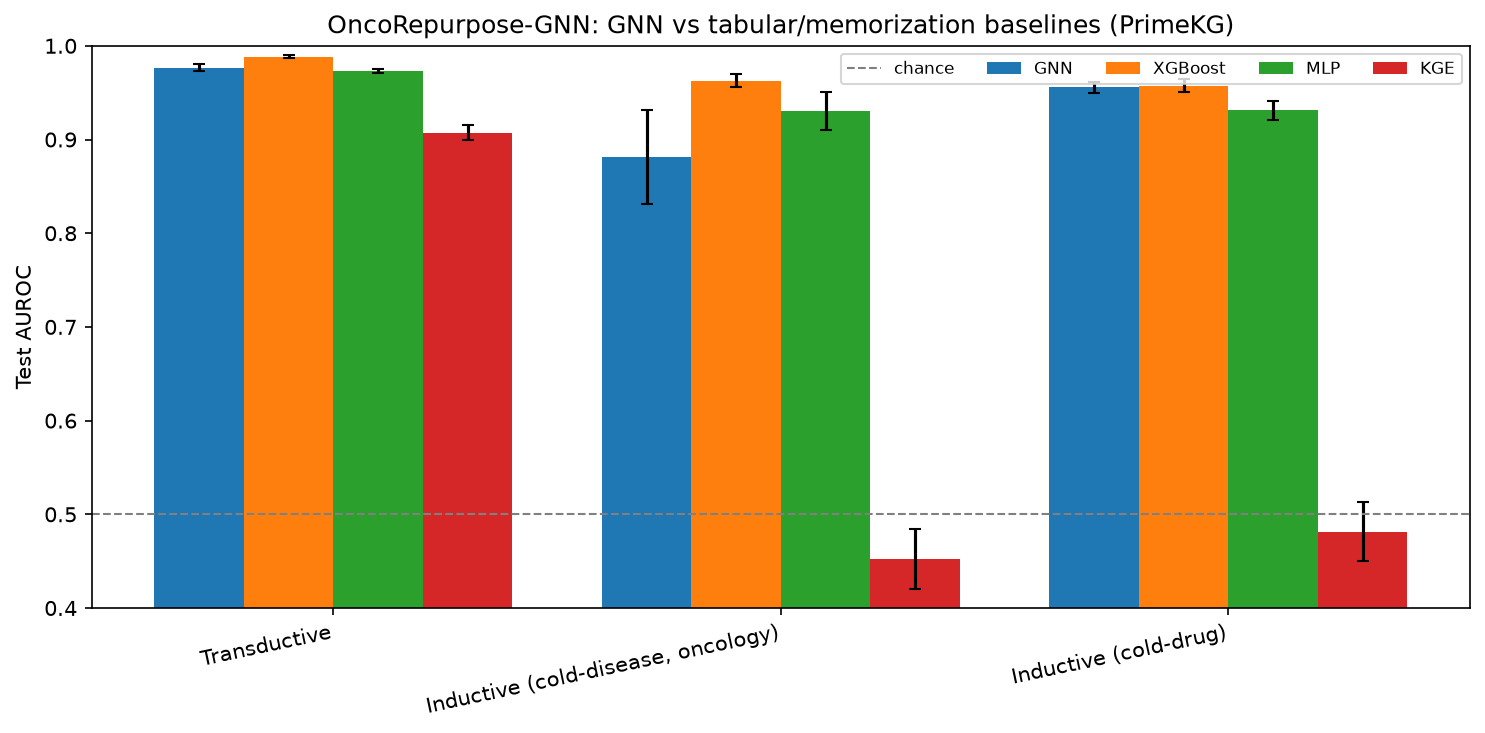
\includegraphics[width=0.86\linewidth]{main_results.png}
\caption{Benchmark AUROC by regime and model (5 seeds, error bars = std). XGBoost (or a
tie) leads everywhere; KGE collapses on the inductive splits.}
\label{fig:bench}
\end{figure}

\subsection{Ablations: where the GNN's ranking signal comes from}
Three ablations locate the GNN's signal (Table~\ref{tab:abl}, Fig.~\ref{fig:abltop}).
Removing all auxiliary topology (\emph{empty}) drops cold-disease AUROC from 0.899 to
0.777, but \emph{shuffling} edges barely hurts (0.879), so the GNN leans on node features
and coarse connectivity more than on specific graph structure. Dropping individual
relation families (drug-protein, disease-protein, pathway) each costs little. And under
non-semantic \emph{structural} features the GNN still does not beat XGBoost
(0.838 vs 0.861), so there is no hidden cold-start ranking win to claim.

\begin{table}[H]
\centering\small
\begin{minipage}[t]{0.48\linewidth}\centering
\begin{tabular}{>{\raggedright\arraybackslash}p{0.5\linewidth} c}
\toprule
\rowcolor{sriblue}\color{white}\textbf{Topology (cold-disease)} & \color{white}\textbf{GNN AUROC}\\
\midrule
\rowcolor{srirow} Intact graph & 0.899\\
Shuffled edges & 0.879\\
\rowcolor{srirow} Empty (features only) & 0.777\\
\bottomrule
\end{tabular}\\[2pt]
{\scriptsize Relation drops: drug-protein 0.934, disease-protein 0.920, pathway 0.933.}
\end{minipage}\hfill
\begin{minipage}[t]{0.48\linewidth}\centering
\begin{tabular}{>{\raggedright\arraybackslash}p{0.34\linewidth} ccc}
\toprule
\rowcolor{sriblue}\color{white}\textbf{Features} & \color{white}\textbf{GNN} & \color{white}\textbf{XGB} & \color{white}\textbf{MLP}\\
\midrule
\rowcolor{srirow} Text (384-d) & 0.889 & \textbf{0.960} & 0.939\\
Structural (23-d) & 0.838 & \textbf{0.861} & 0.830\\
\rowcolor{srirow} Random (64-d) & 0.837 & 0.490 & 0.843\\
\bottomrule
\end{tabular}
\end{minipage}
\caption{Left: topology and relation ablations (3 seeds, cold-disease). Right: feature
ablation (2 seeds). XGBoost's collapse to chance under random features confirms it uses
real signal; the GNN never overtakes it.}
\label{tab:abl}
\end{table}

\begin{figure}[H]
\centering
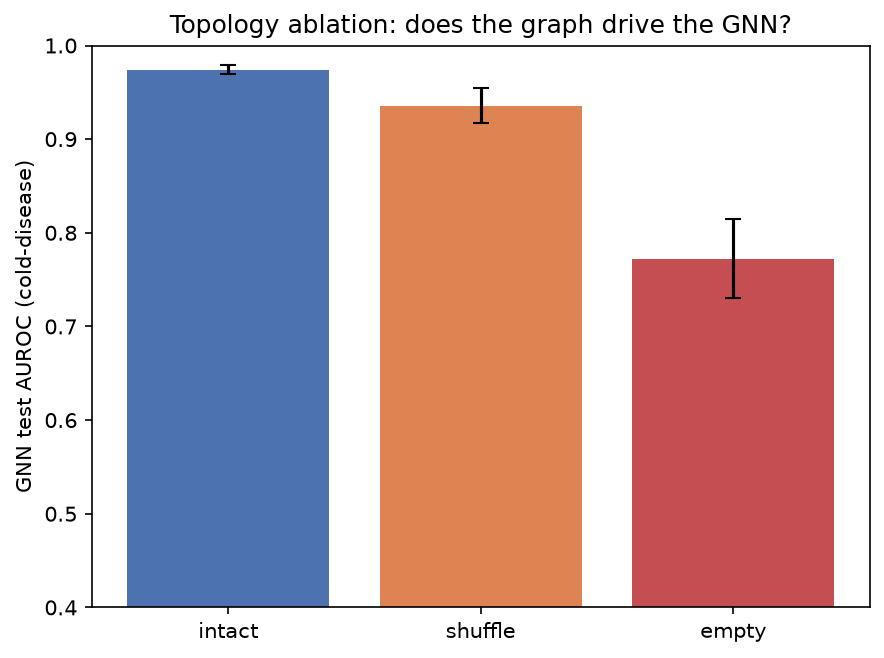
\includegraphics[width=0.72\linewidth]{ablation_topology.png}
\caption{Topology ablation. Erasing structure (\emph{empty}) costs the most; shuffling
edges costs little, indicating the GNN's ranking relies mostly on node features.}
\label{fig:abltop}
\end{figure}

\subsection{Finding 2--3: the graph carries real, discriminative mechanism}
A tabular model cannot produce a traceable mechanism; the graph can (Fig.~\ref{fig:mechpath}).
Over 400 true indications versus 400 random pairs, the mechanism signal separates the two
groups at \textbf{AUROC 0.879} (Table~\ref{tab:sep}, Fig.~\ref{fig:sep}), and the extracted
bridge genes agree with curated DrugMechDB for 211 of 263 covered pairs
(\textbf{0.802}; e.g.\ Methotrexate$\to$\{ATIC, DHFR, TYMS\}, Topotecan$\to$\{TOP1\},
Decitabine$\to$\{DNMT1, DNMT3A\}).

\begin{table}[H]
\centering\small
\begin{tabular}{>{\raggedright\arraybackslash}p{0.40\linewidth} cc}
\toprule
\rowcolor{sriblue}\color{white}\textbf{Metric} & \color{white}\textbf{True} & \color{white}\textbf{Random}\\
\midrule
\rowcolor{srirow} Mean mechanism score & \textbf{1.95} & 0.16\\
Direct-target rate & \textbf{34.0\%} & 0.25\%\\
\rowcolor{srirow} Any mechanistic path & \textbf{81.3\%} & 8.8\%\\
\bottomrule
\end{tabular}
\quad
\raisebox{-2.0\height}{\parbox{0.30\linewidth}{\centering\textbf{Separation AUROC}\\[2pt]
{\Large\color{sriaccent}\textbf{0.879}}}}
\caption{Mechanism paths separate true indications from random pairs. A true indication is
roughly $136\times$ more likely to have a direct drug-target to cancer-gene link.}
\label{tab:sep}
\end{table}

\begin{figure}[H]
\centering
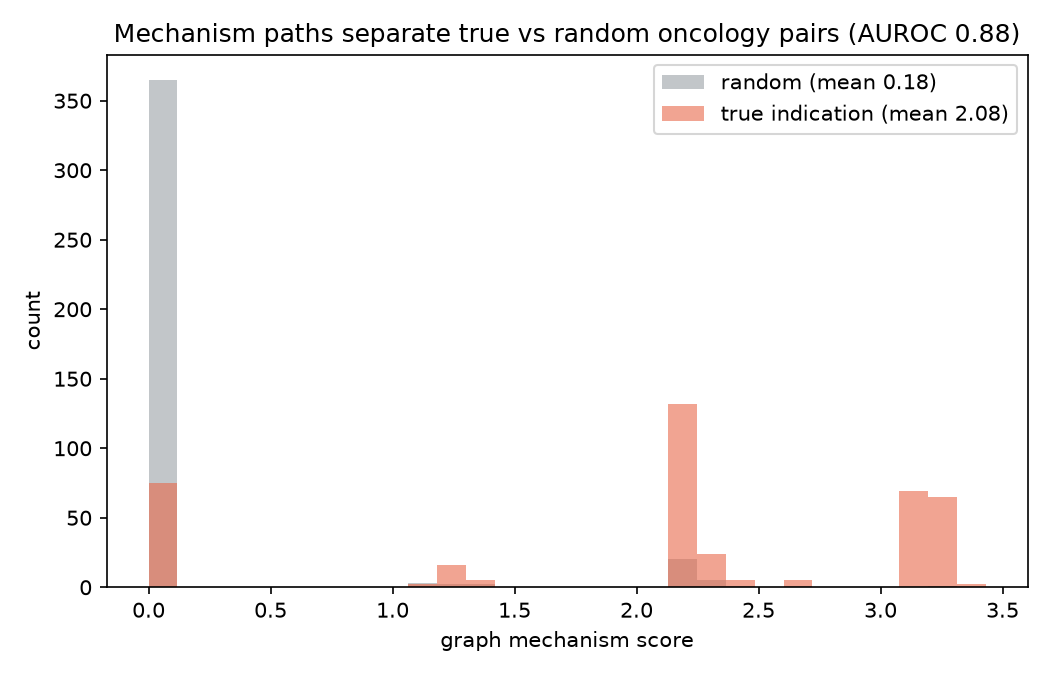
\includegraphics[width=0.74\linewidth]{mechanism_eval.png}
\caption{Distribution of the graph mechanism score for true indications versus random
drug-cancer pairs. Random pairs pile up at zero; true indications spread to high, specific
scores (AUROC 0.879).}
\label{fig:sep}
\end{figure}

\textbf{Robustness to hard negatives.} Separation degrades gracefully as negatives get
harder and only the deliberately adversarial \emph{shared-target} case nears chance
(Table~\ref{tab:hardneg}). An ablation that removes \emph{direct}-target paths still
separates (0.887), so the signal is not merely the most obvious drug-target link.

\begin{table}[H]
\centering\small
\begin{tabular}{>{\raggedright\arraybackslash}p{0.30\linewidth} cccc}
\toprule
\rowcolor{sriblue}\color{white}\textbf{Negatives vs true} & \color{white}\textbf{random} & \color{white}\textbf{oncology-drug} & \color{white}\textbf{degree-matched} & \color{white}\textbf{shared-target}\\
\midrule
\rowcolor{srirow} Separation AUROC & 0.887 & 0.870 & 0.742 & 0.609\\
\bottomrule
\end{tabular}
\caption{Hard-negative stress test (400 vs 400, seed 0). Ablations: full 0.887,
template-only 0.884, no-direct-target 0.887, so indirect mechanisms also separate.}
\label{tab:hardneg}
\end{table}

\textbf{The verifier is a conservative, precise reviewer.} Over 50 true versus 50 random
pairs the language model marks far fewer ``supported'' than a keyword baseline, but those
calls are more trustworthy (Table~\ref{tab:verify}): of its supported calls DrugMechDB
covers, 6/7 are confirmed versus 13/22 for keyword matching.

\begin{table}[H]
\centering\small
\begin{tabular}{>{\raggedright\arraybackslash}p{0.40\linewidth} cc}
\toprule
\rowcolor{sriblue}\color{white}\textbf{} & \color{white}\textbf{Language model} & \color{white}\textbf{Keyword baseline}\\
\midrule
\rowcolor{srirow} True pairs graded ``supported'' & 11 / 50 & 34 / 50\\
Random pairs graded ``supported'' & 1 / 50 & 2 / 50\\
\rowcolor{srirow} \textbf{``Supported'' confirmed by DrugMechDB} & \textbf{0.857} (6/7) & 0.591 (13/22)\\
\bottomrule
\end{tabular}
\caption{Verifier precision (OpenRouter \texttt{gpt-4o-mini}). Small denominators (Wilson
95\% CI roughly 0.49--0.97 for 6/7), so this is a pilot signal. Each verdict carries a
verbatim quote, e.g.\ Topotecan / TOP1: ``a topoisomerase I (TOP1) inhibitor''.}
\label{tab:verify}
\end{table}

\subsection{Finding 4: the graph's one genuine ranking-free edge}
We trained the GNN jointly (Eq.~\ref{eq:infonce}) and asked it to name the curated bridge
gene for held-out cold-disease pairs (3 seeds, $n\approx186$--$260$). Unblinded, a trivial
``the drug's own targets'' baseline dominates because the bridge gene is usually the drug's
direct target. But with that direct edge hidden, the trivial and degree baselines collapse
to about zero while the joint GNN still recovers the gene from indirect structure
(Table~\ref{tab:mechrec}). A link-only GNN scored through the identical head recovers
nothing. Because that link-only head was never trained on the mechanism task, this contrast
isolates the \emph{objective}, not the architecture: the precise claim is that
\emph{joint mechanism supervision creates a recoverable mechanism signal}, which a
link-prediction objective alone does not. We do not claim the architecture by itself could
recover paths.

\begin{table}[H]
\centering\small
\begin{tabular}{>{\raggedright\arraybackslash}p{0.40\linewidth} cc c}
\toprule
\rowcolor{sriblue}\color{white}\textbf{Bridge-gene recovery} & \color{white}\textbf{Unblinded R@10} & \color{white}\textbf{Blinded R@10} & \color{white}\textbf{Blinded MRR}\\
\midrule
\rowcolor{srirow} Joint GNN (link + mechanism) & 0.31 & \textbf{0.25} & \textbf{0.21}\\
Trivial target-lookup & \textbf{0.80} & 0.00 & 0.00\\
\rowcolor{srirow} Link-only GNN (same head, no aux loss) & 0.00 & 0.00 & 0.00\\
Degree prior & 0.02 & 0.02 & 0.02\\
\bottomrule
\end{tabular}
\caption{Mechanism recovery on held-out pairs. When the direct edge is hidden, only the
joint GNN recovers the gene, a small ($\sim$0.25 R@10) but genuine graph-only signal.
Caveat: recovery of \emph{known} mechanism via indirect paths, not de novo discovery, on a
modest sample.}
\label{tab:mechrec}
\end{table}

\subsection{Finding 5 (new): the model is predictive over time}
To test whether the model could have flagged an indication \emph{before} it was
established, we hold out indications by time (cutoff $T=2005$; 350 sampled pairs, 341 years
resolved, 240 past / 101 future; 3 seeds). Trained only on pre-2005 structure, the GNN
ranks the held-out future indications at \textbf{AUROC 0.930} and \textbf{AUPRC 0.707} and
beats the structure-blind control on every metric and seed (Table~\ref{tab:temporal},
Fig.~\ref{fig:temporal}). Unlike the plain link task in Finding 1, the graph adds a small
but consistent edge here, widest on the harder metrics.

\begin{table}[H]
\centering\small
\begin{minipage}[t]{0.52\linewidth}\centering
\begin{tabular}{>{\raggedright\arraybackslash}p{0.34\linewidth} cccc}
\toprule
\rowcolor{sriblue}\color{white}\textbf{$T{=}2005$} & \color{white}\textbf{AUROC} & \color{white}\textbf{AUPRC} & \color{white}\textbf{R@50} & \color{white}\textbf{R@100}\\
\midrule
\rowcolor{srirow} GNN (graph) & \textbf{0.930} & \textbf{0.707} & \textbf{0.393} & \textbf{0.703}\\
MLP (blind) & 0.882 & 0.592 & 0.337 & 0.587\\
\midrule
Graph gain & +0.047 & +0.115 & +0.056 & +0.116\\
\bottomrule
\end{tabular}
\end{minipage}\hfill
\begin{minipage}[t]{0.44\linewidth}
\centering
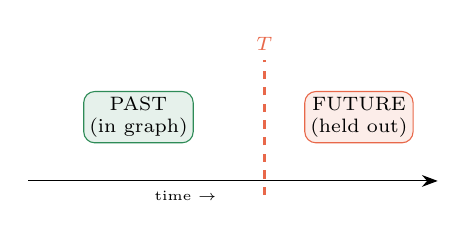
\begin{tikzpicture}[>={Stealth[length=2mm]},font=\scriptsize,xscale=1.0,yscale=0.9]
  \draw[->] (0,0) -- (5.2,0);
  \node[below,font=\tiny] at (2.0,0) {time $\to$};
  \draw[dashed,sriaccent,thick] (3.0,-0.2) -- (3.0,1.7) node[above,sriaccent]{$T$};
  \node[align=center,fill=srigreen!12,draw=srigreen,rounded corners,inner sep=2pt] at (1.4,0.9) {PAST\\(in graph)};
  \node[align=center,fill=sriaccent!12,draw=sriaccent,rounded corners,inner sep=2pt] at (4.2,0.9) {FUTURE\\(held out)};
\end{tikzpicture}
\end{minipage}
\caption{Prospective time-split (mean over 3 seeds). PAST pairs seed the graph; FUTURE
pairs are predicted from pre-$T$ structure only. Caveat: the year proxy is the earliest
literature co-mention, not a regulatory date.}
\label{tab:temporal}
\end{table}

\begin{figure}[H]
\centering
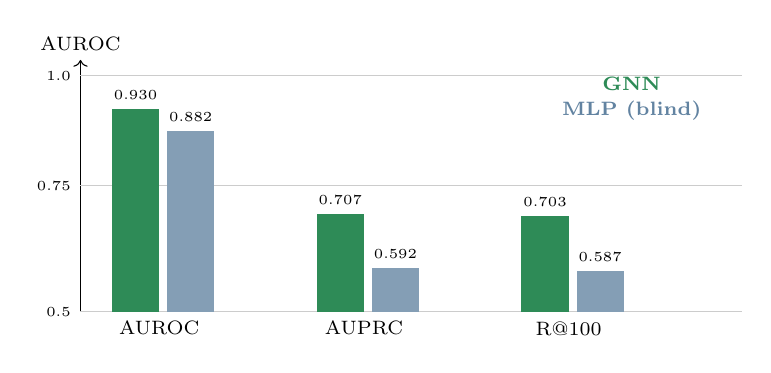
\begin{tikzpicture}[font=\footnotesize]
  \def\bw{0.6}
  % axis
  \draw[->] (0,0) -- (0,3.2) node[above,font=\scriptsize]{AUROC};
  \foreach \y/\yl in {0/0.5,1.6/0.75,3.0/1.0}{\draw[gray!40] (0,\y)--(8.4,\y); \node[left,font=\tiny] at (0,\y){\yl};}
  % map AUROC a in [0.5,1.0] to height (a-0.5)*6
  % GNN bars
  \foreach \i/\g/\m/\lab in {0/0.930/0.882/AUROC, 2.6/0.707/0.592/AUPRC, 5.2/0.703/0.587/{R@100}}{
    \fill[srigreen] (\i+0.4,0) rectangle (\i+0.4+\bw,{(\g-0.5)*6});
    \fill[sriblue!55] (\i+1.1,0) rectangle (\i+1.1+\bw,{(\m-0.5)*6});
    \node[font=\tiny] at (\i+0.7,{(\g-0.5)*6+0.18}){\g};
    \node[font=\tiny] at (\i+1.4,{(\m-0.5)*6+0.18}){\m};
    \node[below,font=\scriptsize] at (\i+1.0,0){\lab};
  }
  \node[srigreen,font=\scriptsize\bfseries] at (7.0,2.9){GNN};
  \node[sriblue!70,font=\scriptsize\bfseries] at (7.0,2.55){MLP (blind)};
\end{tikzpicture}
\caption{Prospective performance: the graph model (green) beats the structure-blind
control (blue) on every metric, with the gap widening on the harder AUPRC and recall@100.}
\label{fig:temporal}
\end{figure}

\textbf{From a metric to named cases.} The AUROC hides what the model actually surfaces, so
we read off, for each held-out \emph{future} indication, where its drug landed when we score
every drug against that cancer using only pre-$T$ structure. Of 101 future indications, the
GNN placed \textbf{11 in the top 50} of $\sim$7{,}956 candidate drugs --- a
\textbf{17.3$\times$} enrichment over a random screen --- against \textbf{1} for the
structure-blind control (1.6$\times$), so the graph yields $11\times$ as many top-50
prospective hits and puts $13.9\%$ of future indications in the top $\sim$1\% versus $1.0\%$
for the control. The hits are recognizable post-cutoff oncology approvals the model had no
indication edge for (Table~\ref{tab:cases}). The graph's edge is concentrated where a
shortlist matters --- the very top of the ranking; across the bulk of pairs the
structure-blind control is competitive, which we report rather than hide. Concretely, over
all 101 future pairs the GNN's \emph{median} rank ($3{,}019$) is actually worse than the
control's ($1{,}482$) and a paired Wilcoxon test does not favor the GNN on overall rank
($p\approx1.0$). The honest claim is therefore narrow and specific: the graph does
\emph{not} rank future indications better on average; it enriches a small, top-priority tail
--- which is exactly the part of the list a repurposing screen actually reads.

\begin{table}[H]
\centering\small
\begin{tabular}{>{\raggedright\arraybackslash}p{0.18\linewidth} >{\raggedright\arraybackslash}p{0.34\linewidth} c c c}
\toprule
\rowcolor{sriblue}\color{white}\textbf{Drug} & \color{white}\textbf{Cancer (future indication)} & \color{white}\textbf{1st lit.\ yr} & \color{white}\textbf{GNN rank} & \color{white}\textbf{MLP rank}\\
\midrule
\rowcolor{srirow} Trabectedin & ovarian carcinoma (several subtypes) & 2006--10 & \textbf{2--5} & 3038\\
Methoxsalen & cutaneous T-cell lymphoma & 2006 & \textbf{10} & 2154\\
Romidepsin & cutaneous T-cell lymphoma & 2008--10 & \textbf{63} & 1726\\
\rowcolor{srirow} Pralatrexate & cutaneous T-cell lymphoma & 2009 & \textbf{321} & 2235\\
Nilotinib & CML, BCR-ABL1 positive & 2006 & \textbf{342} & 1098\\
\rowcolor{srirow} Plerixafor & plasma cell myeloma & 2007 & \textbf{428} & 1797\\
\bottomrule
\end{tabular}
\caption{Prospective named cases (cutoff $T=2005$, single seed). Each indication is first
co-mentioned in the literature after $T$, yet a model trained on pre-$T$ structure alone
ranks the drug near the top of $\sim$7{,}956 candidates for that cancer, far above the
structure-blind control. Ranks are model- and cutoff-dependent; the year is the earliest
Europe PMC co-mention, not a regulatory date.}
\label{tab:cases}
\end{table}

\subsection{Finding 6 (new): the mechanism reasoning is faithful}
Can we trust the mechanism the graph names? For each held-out pair whose bridge gene is a
real drug-target edge we apply Eq.~\ref{eq:faith}: recompute the gene's score with the
full graph, with that pair's curated mechanism edge deleted, and with a random other
target edge of the same drug deleted (316 instances, 2 seeds, no retraining). Removing the
curated edge degrades the bridge gene far more than removing a random one
(Table~\ref{tab:faith}, Fig.~\ref{fig:faith}): a paired Wilcoxon test gives
$p\approx3.6\times10^{-34}$, the model is faithful in 83\% of instances, and the two
populations separate at AUROC 0.835.

\begin{table}[H]
\centering\small
\begin{tabular}{>{\raggedright\arraybackslash}p{0.44\linewidth} cc}
\toprule
\rowcolor{sriblue}\color{white}\textbf{Counterfactual edge removal} & \color{white}\textbf{Score drop} & \color{white}\textbf{Rank drop}\\
\midrule
\rowcolor{srirow} Remove curated mechanism edge & \textbf{0.124} & \textbf{$\sim$211}\\
Remove random target edge (same drug) & $-0.001$ & $\sim$2\\
\midrule
Contrast (faithfulness) & \textbf{0.124} & ---\\
\bottomrule
\end{tabular}
\caption{Faithfulness by counterfactual edge removal (pooled, 316 instances; logit space).
Faithful in 83.3\% of cases; paired Wilcoxon $p\approx3.6\times10^{-34}$; separation AUROC
0.835. Measured on the well-posed population (pairs whose bridge gene is an actual
drug-target edge).}
\label{tab:faith}
\end{table}

\begin{figure}[H]
\centering
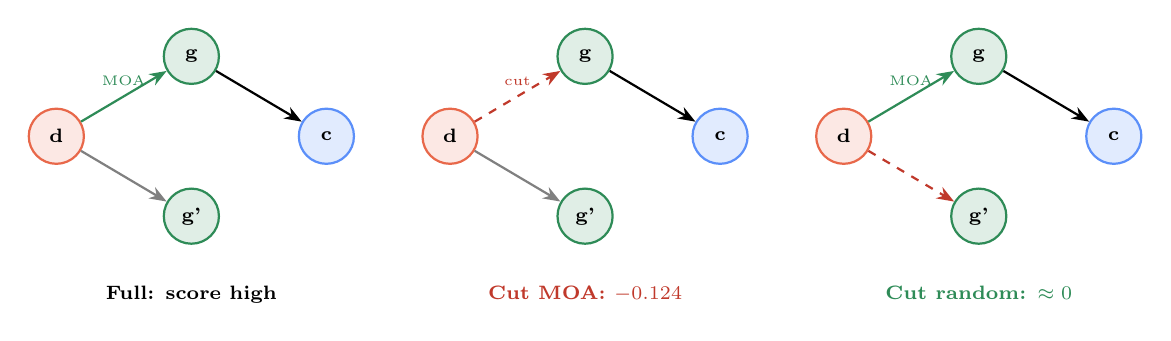
\begin{tikzpicture}[>={Stealth[length=2.2mm]}, node distance=5mm and 12mm,
  drug/.style={circle,draw=nDrug,fill=nDrug!15,thick,font=\scriptsize\bfseries,inner sep=2pt,minimum size=7mm},
  gene/.style={circle,draw=nGene,fill=nGene!15,thick,font=\scriptsize\bfseries,inner sep=2pt,minimum size=7mm},
  dis/.style={circle,draw=nDis,fill=nDis!18,thick,font=\scriptsize\bfseries,inner sep=2pt,minimum size=7mm}]
  % full graph
  \begin{scope}
    \node[drug] (d1){d}; \node[gene,above right=of d1](g1){g}; \node[dis,below right=of g1](c1){c};
    \node[gene,below right=of d1](x1){g'};
    \draw[->,thick,nGene] (d1)--node[above,font=\tiny]{MOA}(g1); \draw[->,thick] (g1)--(c1);
    \draw[->,thick,gray] (d1)--(x1);
    \node[font=\scriptsize\bfseries,below=4mm of x1]{Full: score high};
  \end{scope}
  % remove MOA
  \begin{scope}[xshift=5.0cm]
    \node[drug] (d2){d}; \node[gene,above right=of d2](g2){g}; \node[dis,below right=of g2](c2){c};
    \node[gene,below right=of d2](x2){g'};
    \draw[->,thick,srired,dashed] (d2)--node[above,font=\tiny]{cut}(g2); \draw[->,thick] (g2)--(c2);
    \draw[->,thick,gray] (d2)--(x2);
    \node[srired,font=\scriptsize\bfseries,below=4mm of x2]{Cut MOA: $-0.124$};
  \end{scope}
  % remove random
  \begin{scope}[xshift=10.0cm]
    \node[drug] (d3){d}; \node[gene,above right=of d3](g3){g}; \node[dis,below right=of g3](c3){c};
    \node[gene,below right=of d3](x3){g'};
    \draw[->,thick,nGene] (d3)--node[above,font=\tiny]{MOA}(g3); \draw[->,thick] (g3)--(c3);
    \draw[->,thick,srired,dashed] (d3)--(x3);
    \node[srigreen,font=\scriptsize\bfseries,below=4mm of x3]{Cut random: $\approx 0$};
  \end{scope}
\end{tikzpicture}
\caption{Counterfactual faithfulness. Cutting the curated MOA edge $d\!\to\!g$ collapses
the bridge gene's score; cutting a random other target edge $d\!\to\!g'$ barely changes it.}
\label{fig:faith}
\end{figure}

\subsection{An honest, fully characterized negative: orthogonal trial validation}
\begin{nullbox}
We also asked whether top \emph{novel} predictions (not already PrimeKG indications) appear
as registered oncology trials more than matched controls, and we chased the confounds all
the way down. Top raw-score predictions were not enriched over random (6.7\% versus 7.4\%,
Fisher $p=0.69$). Raw score does track trial existence above chance (AUROC 0.676 over 810
pairs, $p\approx1.5\times10^{-5}$), but a popularity confound is visible immediately: one
broadly-indicated drug (folic acid) accounts for 78\% of the top set's hits.

\emph{Conditioning on the drug} (comparing only cancers for the same drug, which cancels
drug popularity) the model looks strong --- within-drug stratified AUROC $0.821$ ($p=5\times
10^{-4}$ by within-stratum permutation; 49 drugs, 2{,}649 cancer pairs), and for 31/49 drugs
the single highest-scored cancer has a real trial (base rate 0.39, $p=5\times10^{-4}$). But
this still confounds \emph{cancer} popularity (e.g.\ cervical cancer scores $\approx0.998$
for almost every drug and is widely trialed). Removing \emph{both} marginals with a two-way
fixed-effect model --- $\mathrm{score}(d,c)=\mu+\alpha_d+\beta_c+\varepsilon_{dc}$ --- and
testing whether the interaction residual $\varepsilon_{dc}$ predicts a trial gives
\textbf{AUROC $0.475$ (structure-aware permutation $p=0.85$): no signal}. So the apparent
within-drug effect was cancer popularity, not pairwise specificity. The honest reading: raw
deployment scores carry drug- and cancer-level popularity but not the drug$\times$cancer
specificity this registry could corroborate. This is a clean, well-understood negative
rather than a muddy one, and it stands in deliberate contrast to the prospective result
(Finding 5), where specific predictive signal does appear.
\end{nullbox}

% ===========================================================================
\section{Discussion}

The contribution is a disciplined account of where a knowledge graph helps. On plain link
ranking it does not beat a tuned tabular model, and we say so. Its value is the traceable
mechanism a tabular model cannot produce, and this report strengthens that case along the
two axes that matter for a real triage tool. Finding 5 shows the mechanism-aware graph
model is \emph{predictive}: trained only on pre-2005 structure, it ranks post-2005
indications at 0.930 AUROC and beats the structure-blind control, so the signal is not
merely retrospective bookkeeping. Finding 6 shows the mechanism reasoning is
\emph{faithful}: deleting the curated edge, and only that edge, collapses the prediction,
so the explanation reflects the biology the model actually used.

\textbf{Limitations.} The blinded recovery and faithfulness tests are recovery of known
mechanism, not de novo discovery; some samples are modest; the time axis is a literature
proxy; and the orthogonal trial check is a negative, though now a fully characterized one
(the signal is drug/cancer popularity, not pairwise specificity). None of the predictions
are medical advice.

% ===========================================================================
\section{Reproducibility}

Open tools (PyTorch Geometric, scikit-learn, XGBoost) and public data (PrimeKG, Europe
PMC, DrugMechDB, ClinicalTrials.gov). Every reported number has a script and a JSON record
in \texttt{results/}: \texttt{oncorepurpose.json} (Findings 1 + ablations),
\texttt{feature\_ablation.json}, \texttt{mechanism\_eval.json} (Finding 3),
\texttt{hard\_negatives\_eval.json}, \texttt{verify\_llm\_eval.json},
\texttt{mechanism\_recovery\_eval.json} (Finding 4), \texttt{temporal\_split\_eval.json}
and \texttt{prospective\_case\_studies.json} (Finding 5, including the named cases),
\texttt{edge\_faithfulness\_eval.json} (Finding 6), and \texttt{clinicaltrials\_validation.json}
with \texttt{clinicaltrials\_deconfounded.json} (the characterized negative). An eight-part Colab notebook track
reproduces the pipeline end to end (Part 4 is fully self-contained; Parts 7--8 cover the prospective
named cases and the popularity-deconfounded check). All predictions are
hypothesis-generating research, not medical advice.

% ===========================================================================
\begin{thebibliography}{9}
\small
\bibitem{txgnn} Huang K, Chandak P, et al. \textit{A foundation model for
clinician-centered drug repurposing (TxGNN)}. Nature Medicine, 2024.
\bibitem{primekg} Chandak P, Huang K, Zitnik M. \textit{Building a knowledge graph to
enable precision medicine (PrimeKG)}. Scientific Data, 2023.
\bibitem{kgmlxdtd} \textit{KGML-xDTD: a knowledge graph-based framework for drug treatment
prediction and mechanism description}. 2023.
\bibitem{decagon} Zitnik M, Agrawal M, Leskovec J. \textit{Modeling polypharmacy side
effects with graph convolutional networks (Decagon)}. Bioinformatics, 2018.
\bibitem{drugmechdb} Mayers M, et al. \textit{DrugMechDB: a curated database of drug
mechanism paths}. 2022.
\bibitem{sage} Hamilton W, Ying R, Leskovec J. \textit{Inductive representation learning on
large graphs (GraphSAGE)}. NeurIPS, 2017.
\end{thebibliography}

\end{document}
